\begin{figure}[t]
\centering
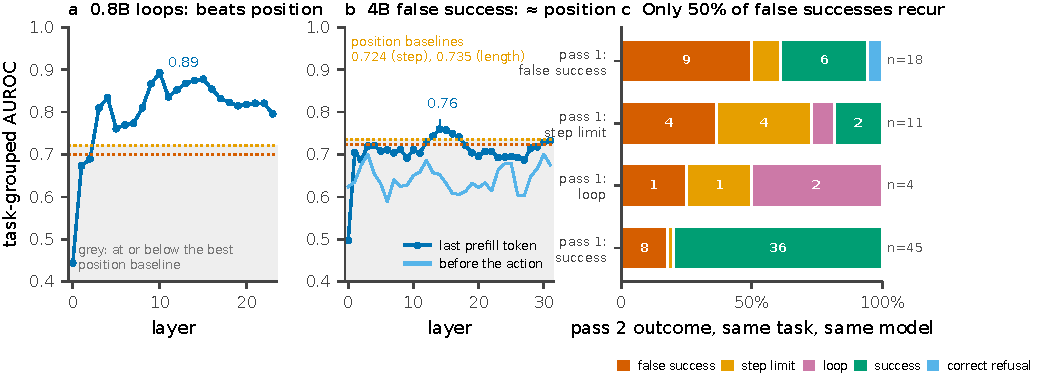
\includegraphics[width=\linewidth]{figs/traps.pdf}
\caption{\textbf{Two of the three traps.} (a)~Holo-3.1-0.8B, MiniWoB++: a loop direction separates loop steps far above the step-index (red) and context-length (orange) baselines, with task-grouped cross-validation. It still fails every causal test (\S\ref{sec:mw}). (b)~Holo-3.1-4B, OSWorld, official analysis on both passes (\ofPos{} \fsp, \ofNeg{} \fsm, \ofTasks{} tasks): the false-versus-true completion direction stays within noise of the position baselines at its best layer (\ofResidAuc{} against \ofBaseStep{} and \ofBaseCtx, standard error \ofResidSe), with or without position controlled (Table~\ref{tab:fs-auc}). The grey band marks AUROCs at or below the best baseline. (c)~The unmodified 4B run twice on the same tasks (\rtmBoth{} tasks scored in both passes). Only \rtmFsAgain{} of \rtmFsN{} pass-1 false successes recur, against \rtmSuccAgain{} of \rtmSuccN{} pass-1 successes.}
\label{fig:traps}
\end{figure}
